\section{Referencia del Archivo /media/docs/progra/c++/compiladores1/proy2/godzilla/src/constantes.h}
\label{constantes_8h}\index{/media/docs/progra/c++/compiladores1/proy2/godzilla/src/constantes.h@{/media/docs/progra/c++/compiladores1/proy2/godzilla/src/constantes.h}}
Constantes utilizadas por el arbol de sintaxis abstracta. 



Este gr\'{a}fico muestra que archivos directa o indirectamente incluyen a este archivo:\begin{figure}[H]
\begin{center}
\leavevmode
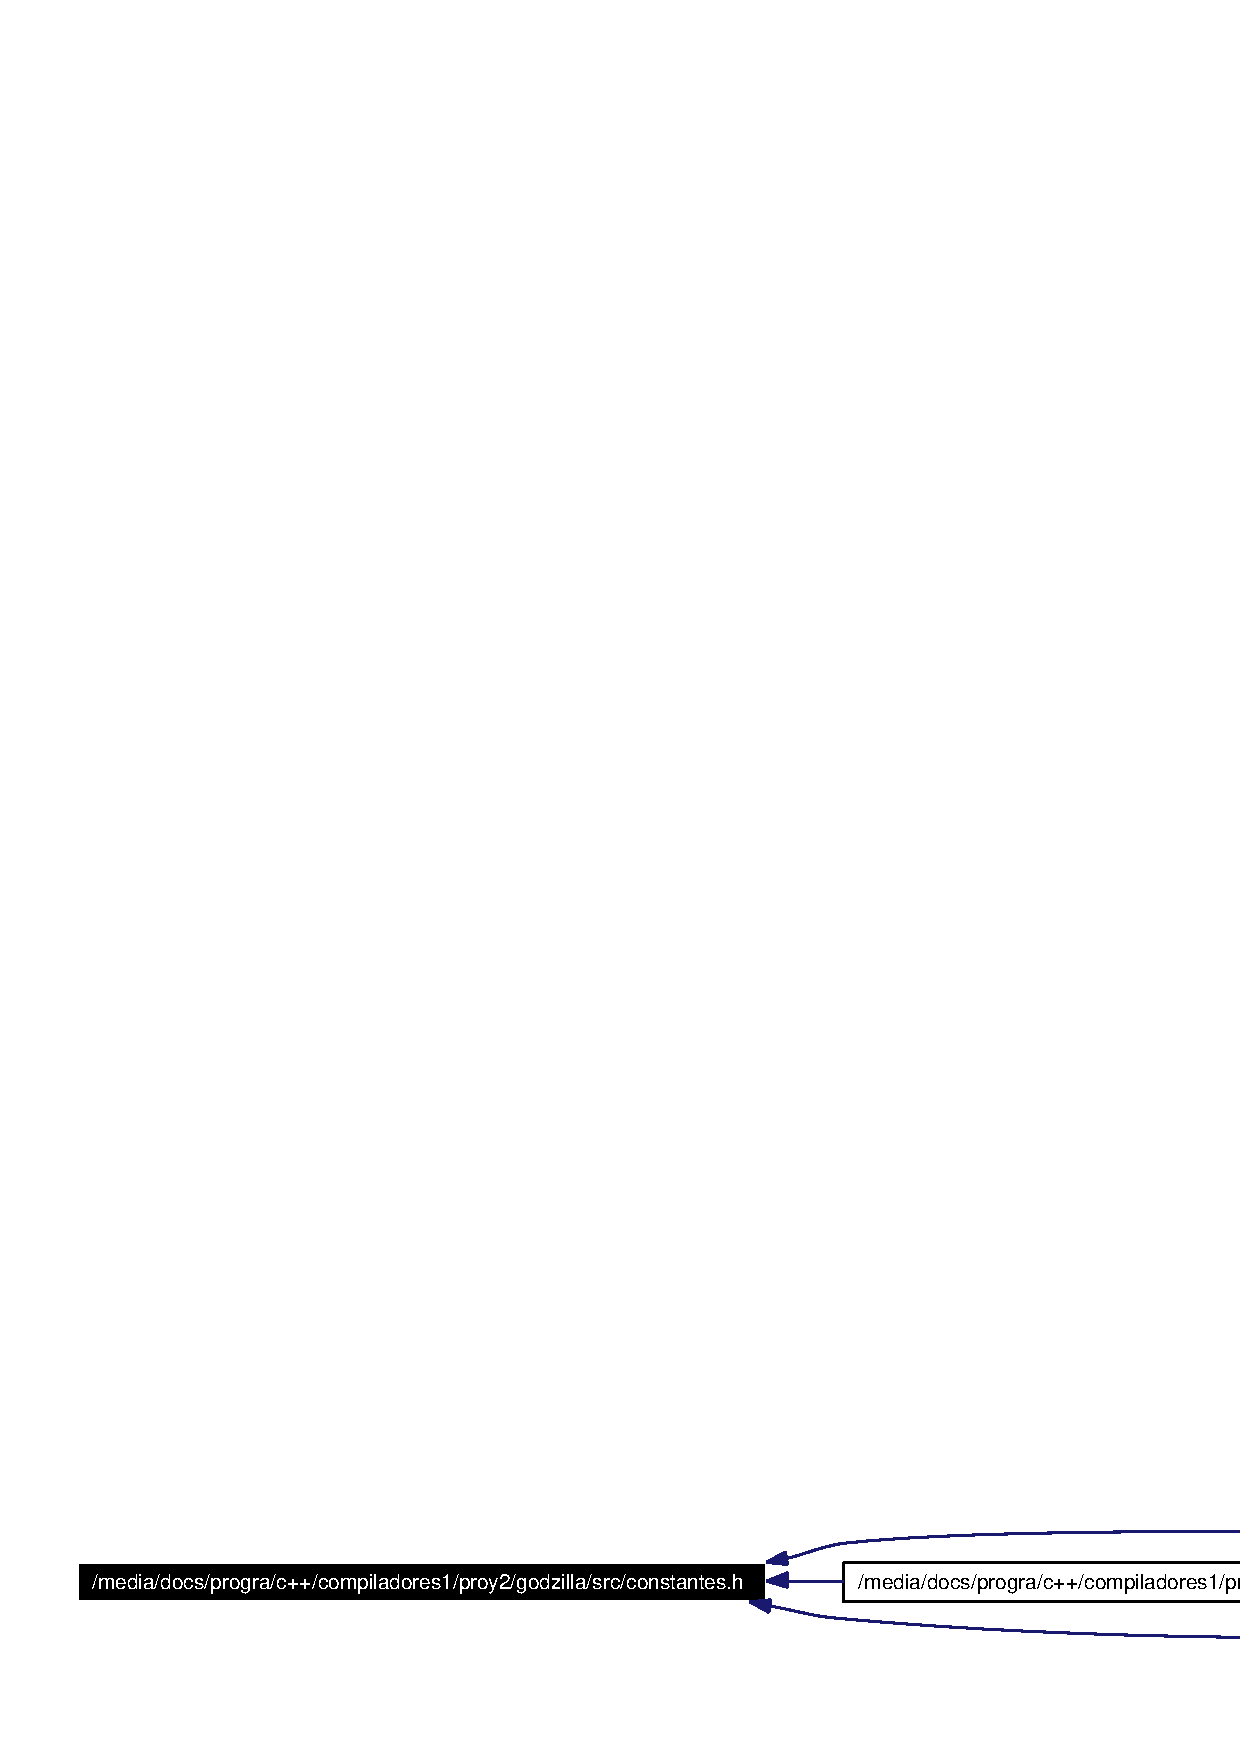
\includegraphics[width=420pt]{constantes_8h__dep__incl}
\end{center}
\end{figure}
\subsection*{Definiciones}
\begin{CompactItemize}
\item 
\#define {\bf T\_\-ERROR}~-1
\item 
\#define {\bf T\_\-FALSE}~0
\item 
\#define {\bf T\_\-TRUE}~1
\item 
\#define {\bf T\_\-CONSTANTE}~1000
\item 
\#define {\bf T\_\-VARIABLE}~1001
\item 
\#define {\bf T\_\-NUMERO}~1002
\item 
\#define {\bf T\_\-IDENTIFICADOR}~1003
\item 
\#define {\bf T\_\-OPERACION}~1004
\item 
\#define {\bf T\_\-EXPR}~1005
\item 
\#define {\bf T\_\-ASIGNACION}~1006
\item 
\#define {\bf T\_\-SENTENCIA}~1007
\item 
\#define {\bf T\_\-DECLARACION}~1008
\item 
\#define {\bf T\_\-IF}~1009
\item 
\#define {\bf T\_\-WHILE}~1010
\item 
\#define {\bf T\_\-FOR}~1011
\item 
\#define {\bf T\_\-TOKEN}~1012
\item 
\#define {\bf T\_\-CALL}~1013
\item 
\#define {\bf T\_\-CADENA}~1015
\item 
\#define {\bf OP\_\-OR}~1016
\item 
\#define {\bf OP\_\-AND}~1017
\item 
\#define {\bf OP\_\-LT}~1018
\item 
\#define {\bf OP\_\-LET}~1019
\item 
\#define {\bf OP\_\-EQ}~1020
\item 
\#define {\bf OP\_\-NEQ}~1021
\item 
\#define {\bf OP\_\-GT}~1022
\item 
\#define {\bf OP\_\-GET}~1023
\item 
\#define {\bf OP\_\-SUMA}~1024
\item 
\#define {\bf OP\_\-RESTA}~1025
\item 
\#define {\bf OP\_\-MULT}~1026
\item 
\#define {\bf OP\_\-DIV}~1027
\item 
\#define {\bf T\_\-INTEGER}~1028
\item 
\#define {\bf T\_\-BOOLEAN}~1029
\item 
\#define {\bf T\_\-STRING}~1030
\item 
\#define {\bf T\_\-LITERAL}~1031
\item 
\#define {\bf T\_\-PRINTCALL}~1032
\item 
\#define {\bf T\_\-PRINTSYMCALL}~1033
\end{CompactItemize}


\subsection{Descripci\'{o}n detallada}
Constantes utilizadas por el arbol de sintaxis abstracta. 



Definici\'{o}n en el archivo {\bf constantes.h}.

\subsection{Documentaci\'{o}n de las definiciones}
\index{constantes.h@{constantes.h}!OP_AND@{OP\_\-AND}}
\index{OP_AND@{OP\_\-AND}!constantes.h@{constantes.h}}
\subsubsection{\setlength{\rightskip}{0pt plus 5cm}\#define OP\_\-AND~1017}\label{constantes_8h_a19}




Definici\'{o}n en la l\'{\i}nea 30 del archivo constantes.h.

Referenciado por evaluar\-Operacion().\index{constantes.h@{constantes.h}!OP_DIV@{OP\_\-DIV}}
\index{OP_DIV@{OP\_\-DIV}!constantes.h@{constantes.h}}
\subsubsection{\setlength{\rightskip}{0pt plus 5cm}\#define OP\_\-DIV~1027}\label{constantes_8h_a29}




Definici\'{o}n en la l\'{\i}nea 40 del archivo constantes.h.

Referenciado por evaluar\-Operacion().\index{constantes.h@{constantes.h}!OP_EQ@{OP\_\-EQ}}
\index{OP_EQ@{OP\_\-EQ}!constantes.h@{constantes.h}}
\subsubsection{\setlength{\rightskip}{0pt plus 5cm}\#define OP\_\-EQ~1020}\label{constantes_8h_a22}




Definici\'{o}n en la l\'{\i}nea 33 del archivo constantes.h.

Referenciado por evaluar\-Operacion().\index{constantes.h@{constantes.h}!OP_GET@{OP\_\-GET}}
\index{OP_GET@{OP\_\-GET}!constantes.h@{constantes.h}}
\subsubsection{\setlength{\rightskip}{0pt plus 5cm}\#define OP\_\-GET~1023}\label{constantes_8h_a25}




Definici\'{o}n en la l\'{\i}nea 36 del archivo constantes.h.

Referenciado por evaluar\-Operacion().\index{constantes.h@{constantes.h}!OP_GT@{OP\_\-GT}}
\index{OP_GT@{OP\_\-GT}!constantes.h@{constantes.h}}
\subsubsection{\setlength{\rightskip}{0pt plus 5cm}\#define OP\_\-GT~1022}\label{constantes_8h_a24}




Definici\'{o}n en la l\'{\i}nea 35 del archivo constantes.h.

Referenciado por evaluar\-Operacion().\index{constantes.h@{constantes.h}!OP_LET@{OP\_\-LET}}
\index{OP_LET@{OP\_\-LET}!constantes.h@{constantes.h}}
\subsubsection{\setlength{\rightskip}{0pt plus 5cm}\#define OP\_\-LET~1019}\label{constantes_8h_a21}




Definici\'{o}n en la l\'{\i}nea 32 del archivo constantes.h.

Referenciado por evaluar\-Operacion().\index{constantes.h@{constantes.h}!OP_LT@{OP\_\-LT}}
\index{OP_LT@{OP\_\-LT}!constantes.h@{constantes.h}}
\subsubsection{\setlength{\rightskip}{0pt plus 5cm}\#define OP\_\-LT~1018}\label{constantes_8h_a20}




Definici\'{o}n en la l\'{\i}nea 31 del archivo constantes.h.

Referenciado por evaluar\-Operacion().\index{constantes.h@{constantes.h}!OP_MULT@{OP\_\-MULT}}
\index{OP_MULT@{OP\_\-MULT}!constantes.h@{constantes.h}}
\subsubsection{\setlength{\rightskip}{0pt plus 5cm}\#define OP\_\-MULT~1026}\label{constantes_8h_a28}




Definici\'{o}n en la l\'{\i}nea 39 del archivo constantes.h.

Referenciado por evaluar\-Operacion().\index{constantes.h@{constantes.h}!OP_NEQ@{OP\_\-NEQ}}
\index{OP_NEQ@{OP\_\-NEQ}!constantes.h@{constantes.h}}
\subsubsection{\setlength{\rightskip}{0pt plus 5cm}\#define OP\_\-NEQ~1021}\label{constantes_8h_a23}




Definici\'{o}n en la l\'{\i}nea 34 del archivo constantes.h.

Referenciado por evaluar\-Operacion().\index{constantes.h@{constantes.h}!OP_OR@{OP\_\-OR}}
\index{OP_OR@{OP\_\-OR}!constantes.h@{constantes.h}}
\subsubsection{\setlength{\rightskip}{0pt plus 5cm}\#define OP\_\-OR~1016}\label{constantes_8h_a18}




Definici\'{o}n en la l\'{\i}nea 29 del archivo constantes.h.

Referenciado por evaluar\-Operacion().\index{constantes.h@{constantes.h}!OP_RESTA@{OP\_\-RESTA}}
\index{OP_RESTA@{OP\_\-RESTA}!constantes.h@{constantes.h}}
\subsubsection{\setlength{\rightskip}{0pt plus 5cm}\#define OP\_\-RESTA~1025}\label{constantes_8h_a27}




Definici\'{o}n en la l\'{\i}nea 38 del archivo constantes.h.

Referenciado por evaluar\-Operacion().\index{constantes.h@{constantes.h}!OP_SUMA@{OP\_\-SUMA}}
\index{OP_SUMA@{OP\_\-SUMA}!constantes.h@{constantes.h}}
\subsubsection{\setlength{\rightskip}{0pt plus 5cm}\#define OP\_\-SUMA~1024}\label{constantes_8h_a26}




Definici\'{o}n en la l\'{\i}nea 37 del archivo constantes.h.

Referenciado por evaluar\-Operacion().\index{constantes.h@{constantes.h}!T_ASIGNACION@{T\_\-ASIGNACION}}
\index{T_ASIGNACION@{T\_\-ASIGNACION}!constantes.h@{constantes.h}}
\subsubsection{\setlength{\rightskip}{0pt plus 5cm}\#define T\_\-ASIGNACION~1006}\label{constantes_8h_a9}




Definici\'{o}n en la l\'{\i}nea 20 del archivo constantes.h.

Referenciado por borrar\-Sentencias(), evaluar\-Asignacion(), evaluar\-Sentencia(), insertar\-Asignacion(), y insertar\-Sentencia().\index{constantes.h@{constantes.h}!T_BOOLEAN@{T\_\-BOOLEAN}}
\index{T_BOOLEAN@{T\_\-BOOLEAN}!constantes.h@{constantes.h}}
\subsubsection{\setlength{\rightskip}{0pt plus 5cm}\#define T\_\-BOOLEAN~1029}\label{constantes_8h_a31}




Definici\'{o}n en la l\'{\i}nea 42 del archivo constantes.h.

Referenciado por evaluar\-And(), evaluar\-Asignacion(), evaluar\-EQ(), evaluar\-Expresion(), evaluar\-GET(), evaluar\-GT(), evaluar\-If(), evaluar\-LET(), evaluar\-LT(), evaluar\-NEQ(), evaluar\-Or(), evaluar\-While(), imprimir\-Tokens(), insertar\-Simbolo(), y print\-Symtab\-File().\index{constantes.h@{constantes.h}!T_CADENA@{T\_\-CADENA}}
\index{T_CADENA@{T\_\-CADENA}!constantes.h@{constantes.h}}
\subsubsection{\setlength{\rightskip}{0pt plus 5cm}\#define T\_\-CADENA~1015}\label{constantes_8h_a17}




Definici\'{o}n en la l\'{\i}nea 28 del archivo constantes.h.

Referenciado por borrar\-Tokens(), imprimir\-Tokens(), y insertar\-Token().\index{constantes.h@{constantes.h}!T_CALL@{T\_\-CALL}}
\index{T_CALL@{T\_\-CALL}!constantes.h@{constantes.h}}
\subsubsection{\setlength{\rightskip}{0pt plus 5cm}\#define T\_\-CALL~1013}\label{constantes_8h_a16}




Definici\'{o}n en la l\'{\i}nea 27 del archivo constantes.h.

Referenciado por borrar\-Sentencias(), evaluar\-Print\-Call(), evaluar\-Sentencia(), insertar\-Llamada(), insertar\-Llamada\-Sym\-Tab(), y insertar\-Sentencia().\index{constantes.h@{constantes.h}!T_CONSTANTE@{T\_\-CONSTANTE}}
\index{T_CONSTANTE@{T\_\-CONSTANTE}!constantes.h@{constantes.h}}
\subsubsection{\setlength{\rightskip}{0pt plus 5cm}\#define T\_\-CONSTANTE~1000}\label{constantes_8h_a3}




Definici\'{o}n en la l\'{\i}nea 14 del archivo constantes.h.

Referenciado por borrar\-Expresion(), evaluar\-Expresion(), insertar\-Constante(), y insertar\-Expresion().\index{constantes.h@{constantes.h}!T_DECLARACION@{T\_\-DECLARACION}}
\index{T_DECLARACION@{T\_\-DECLARACION}!constantes.h@{constantes.h}}
\subsubsection{\setlength{\rightskip}{0pt plus 5cm}\#define T\_\-DECLARACION~1008}\label{constantes_8h_a11}




Definici\'{o}n en la l\'{\i}nea 22 del archivo constantes.h.

Referenciado por borrar\-Sentencias(), evaluar\-Declaracion(), evaluar\-Sentencia(), insertar\-Declaracion(), y insertar\-Sentencia().\index{constantes.h@{constantes.h}!T_ERROR@{T\_\-ERROR}}
\index{T_ERROR@{T\_\-ERROR}!constantes.h@{constantes.h}}
\subsubsection{\setlength{\rightskip}{0pt plus 5cm}\#define T\_\-ERROR~-1}\label{constantes_8h_a0}




Definici\'{o}n en la l\'{\i}nea 11 del archivo constantes.h.

Referenciado por evaluar\-Sentencia(), y insertar\-Sentencia().\index{constantes.h@{constantes.h}!T_EXPR@{T\_\-EXPR}}
\index{T_EXPR@{T\_\-EXPR}!constantes.h@{constantes.h}}
\subsubsection{\setlength{\rightskip}{0pt plus 5cm}\#define T\_\-EXPR~1005}\label{constantes_8h_a8}




Definici\'{o}n en la l\'{\i}nea 19 del archivo constantes.h.

Referenciado por evaluar\-Expresion(), insertar\-Cadena(), y insertar\-Expresion().\index{constantes.h@{constantes.h}!T_FALSE@{T\_\-FALSE}}
\index{T_FALSE@{T\_\-FALSE}!constantes.h@{constantes.h}}
\subsubsection{\setlength{\rightskip}{0pt plus 5cm}\#define T\_\-FALSE~0}\label{constantes_8h_a1}




Definici\'{o}n en la l\'{\i}nea 12 del archivo constantes.h.

Referenciado por evaluar\-And(), evaluar\-EQ(), evaluar\-GET(), evaluar\-GT(), evaluar\-If(), evaluar\-LET(), evaluar\-LT(), evaluar\-NEQ(), evaluar\-Or(), y evaluar\-While().\index{constantes.h@{constantes.h}!T_FOR@{T\_\-FOR}}
\index{T_FOR@{T\_\-FOR}!constantes.h@{constantes.h}}
\subsubsection{\setlength{\rightskip}{0pt plus 5cm}\#define T\_\-FOR~1011}\label{constantes_8h_a14}




Definici\'{o}n en la l\'{\i}nea 25 del archivo constantes.h.

Referenciado por borrar\-Sentencias(), evaluar\-For(), evaluar\-Sentencia(), insertar\-Ciclo\-For(), y insertar\-Sentencia().\index{constantes.h@{constantes.h}!T_IDENTIFICADOR@{T\_\-IDENTIFICADOR}}
\index{T_IDENTIFICADOR@{T\_\-IDENTIFICADOR}!constantes.h@{constantes.h}}
\subsubsection{\setlength{\rightskip}{0pt plus 5cm}\#define T\_\-IDENTIFICADOR~1003}\label{constantes_8h_a6}




Definici\'{o}n en la l\'{\i}nea 17 del archivo constantes.h.

Referenciado por imprimir\-Tokens(), y insertar\-Token().\index{constantes.h@{constantes.h}!T_IF@{T\_\-IF}}
\index{T_IF@{T\_\-IF}!constantes.h@{constantes.h}}
\subsubsection{\setlength{\rightskip}{0pt plus 5cm}\#define T\_\-IF~1009}\label{constantes_8h_a12}




Definici\'{o}n en la l\'{\i}nea 23 del archivo constantes.h.

Referenciado por borrar\-Sentencias(), evaluar\-If(), evaluar\-Sentencia(), insertar\-Enunciado\-If(), y insertar\-Sentencia().\index{constantes.h@{constantes.h}!T_INTEGER@{T\_\-INTEGER}}
\index{T_INTEGER@{T\_\-INTEGER}!constantes.h@{constantes.h}}
\subsubsection{\setlength{\rightskip}{0pt plus 5cm}\#define T\_\-INTEGER~1028}\label{constantes_8h_a30}




Definici\'{o}n en la l\'{\i}nea 41 del archivo constantes.h.

Referenciado por evaluar\-Asignacion(), evaluar\-Div(), evaluar\-EQ(), evaluar\-Expresion(), evaluar\-For(), evaluar\-GET(), evaluar\-GT(), evaluar\-LET(), evaluar\-LT(), evaluar\-Mult(), evaluar\-NEQ(), evaluar\-Resta(), evaluar\-Suma(), imprimir\-Tokens(), insertar\-Simbolo(), insertar\-Token(), y print\-Symtab\-File().\index{constantes.h@{constantes.h}!T_LITERAL@{T\_\-LITERAL}}
\index{T_LITERAL@{T\_\-LITERAL}!constantes.h@{constantes.h}}
\subsubsection{\setlength{\rightskip}{0pt plus 5cm}\#define T\_\-LITERAL~1031}\label{constantes_8h_a33}




Definici\'{o}n en la l\'{\i}nea 44 del archivo constantes.h.

Referenciado por borrar\-Expresion(), evaluar\-Expresion(), y insertar\-Cadena().\index{constantes.h@{constantes.h}!T_NUMERO@{T\_\-NUMERO}}
\index{T_NUMERO@{T\_\-NUMERO}!constantes.h@{constantes.h}}
\subsubsection{\setlength{\rightskip}{0pt plus 5cm}\#define T\_\-NUMERO~1002}\label{constantes_8h_a5}




Definici\'{o}n en la l\'{\i}nea 16 del archivo constantes.h.

Referenciado por evaluar\-Asignacion(), evaluar\-Expresion(), imprimir\-Tokens(), y insertar\-Token().\index{constantes.h@{constantes.h}!T_OPERACION@{T\_\-OPERACION}}
\index{T_OPERACION@{T\_\-OPERACION}!constantes.h@{constantes.h}}
\subsubsection{\setlength{\rightskip}{0pt plus 5cm}\#define T\_\-OPERACION~1004}\label{constantes_8h_a7}




Definici\'{o}n en la l\'{\i}nea 18 del archivo constantes.h.

Referenciado por borrar\-Expresion(), evaluar\-And(), evaluar\-Div(), evaluar\-Expresion(), evaluar\-GET(), evaluar\-GT(), evaluar\-LET(), evaluar\-LT(), evaluar\-Mult(), evaluar\-Or(), evaluar\-Resta(), evaluar\-Suma(), insertar\-Expresion(), y insertar\-Operacion().\index{constantes.h@{constantes.h}!T_PRINTCALL@{T\_\-PRINTCALL}}
\index{T_PRINTCALL@{T\_\-PRINTCALL}!constantes.h@{constantes.h}}
\subsubsection{\setlength{\rightskip}{0pt plus 5cm}\#define T\_\-PRINTCALL~1032}\label{constantes_8h_a34}




Definici\'{o}n en la l\'{\i}nea 46 del archivo constantes.h.

Referenciado por evaluar\-Print\-Call(), y insertar\-Llamada().\index{constantes.h@{constantes.h}!T_PRINTSYMCALL@{T\_\-PRINTSYMCALL}}
\index{T_PRINTSYMCALL@{T\_\-PRINTSYMCALL}!constantes.h@{constantes.h}}
\subsubsection{\setlength{\rightskip}{0pt plus 5cm}\#define T\_\-PRINTSYMCALL~1033}\label{constantes_8h_a35}




Definici\'{o}n en la l\'{\i}nea 47 del archivo constantes.h.

Referenciado por insertar\-Llamada\-Sym\-Tab().\index{constantes.h@{constantes.h}!T_SENTENCIA@{T\_\-SENTENCIA}}
\index{T_SENTENCIA@{T\_\-SENTENCIA}!constantes.h@{constantes.h}}
\subsubsection{\setlength{\rightskip}{0pt plus 5cm}\#define T\_\-SENTENCIA~1007}\label{constantes_8h_a10}




Definici\'{o}n en la l\'{\i}nea 21 del archivo constantes.h.

Referenciado por crear\-Raiz(), error(), insertar\-Sentencia(), y recorrer\-Sentencia().\index{constantes.h@{constantes.h}!T_STRING@{T\_\-STRING}}
\index{T_STRING@{T\_\-STRING}!constantes.h@{constantes.h}}
\subsubsection{\setlength{\rightskip}{0pt plus 5cm}\#define T\_\-STRING~1030}\label{constantes_8h_a32}




Definici\'{o}n en la l\'{\i}nea 43 del archivo constantes.h.

Referenciado por borrar\-Nodos(), borrar\-Tokens(), evaluar\-EQ(), evaluar\-Expresion(), evaluar\-NEQ(), evaluar\-Suma(), imprimir\-Tokens(), insertar\-Simbolo(), insertar\-Token(), y print\-Symtab\-File().\index{constantes.h@{constantes.h}!T_TOKEN@{T\_\-TOKEN}}
\index{T_TOKEN@{T\_\-TOKEN}!constantes.h@{constantes.h}}
\subsubsection{\setlength{\rightskip}{0pt plus 5cm}\#define T\_\-TOKEN~1012}\label{constantes_8h_a15}




Definici\'{o}n en la l\'{\i}nea 26 del archivo constantes.h.

Referenciado por imprimir\-Tokens(), y insertar\-Token().\index{constantes.h@{constantes.h}!T_TRUE@{T\_\-TRUE}}
\index{T_TRUE@{T\_\-TRUE}!constantes.h@{constantes.h}}
\subsubsection{\setlength{\rightskip}{0pt plus 5cm}\#define T\_\-TRUE~1}\label{constantes_8h_a2}




Definici\'{o}n en la l\'{\i}nea 13 del archivo constantes.h.

Referenciado por evaluar\-And(), evaluar\-EQ(), evaluar\-GET(), evaluar\-GT(), evaluar\-If(), evaluar\-LET(), evaluar\-LT(), evaluar\-NEQ(), evaluar\-Or(), y evaluar\-While().\index{constantes.h@{constantes.h}!T_VARIABLE@{T\_\-VARIABLE}}
\index{T_VARIABLE@{T\_\-VARIABLE}!constantes.h@{constantes.h}}
\subsubsection{\setlength{\rightskip}{0pt plus 5cm}\#define T\_\-VARIABLE~1001}\label{constantes_8h_a4}




Definici\'{o}n en la l\'{\i}nea 15 del archivo constantes.h.

Referenciado por borrar\-Expresion(), evaluar\-Expresion(), insertar\-Expresion(), y insertar\-Variable().\index{constantes.h@{constantes.h}!T_WHILE@{T\_\-WHILE}}
\index{T_WHILE@{T\_\-WHILE}!constantes.h@{constantes.h}}
\subsubsection{\setlength{\rightskip}{0pt plus 5cm}\#define T\_\-WHILE~1010}\label{constantes_8h_a13}




Definici\'{o}n en la l\'{\i}nea 24 del archivo constantes.h.

Referenciado por borrar\-Sentencias(), evaluar\-Sentencia(), evaluar\-While(), insertar\-Ciclo\-While(), y insertar\-Sentencia().